\documentclass[12pt,a4,oneside,usenames,dvipsnames]{book}
  \usepackage{polyglossia}
  \usepackage{fontspec}
  \setmainlanguage{english}
  \setotherlanguage{greek}
  \setmainfont[Scale=0.8]{Avara}
  \usepackage{unicode-math}
  %\setmathfont{Latin Modern Math}
  \setmathfont{TeX Gyre Pagella Math}
  \newfontfamily\pixel[Scale=1]{terminal-grotesque.ttf}
  \newfontfamily\fira[Scale=1]{Fira Sans}
  \usepackage{microtype}
  \usepackage{dot2texi}
  \usepackage{hyperref}
\hypersetup{
    unicode,
    verbose=false,
    pdfpagelayout=TwoColumnRight,
    bookmarksopen,
    colorlinks,
    citecolor=black,
    filecolor=black,
    linkcolor=black,
    urlcolor=black
}
  \usepackage{microtype}
  \usepackage[noclrdblpg]{colophon}
  \usepackage{bookmark}
  \usepackage{amsmath}
  \usepackage{float}
  \usepackage{skeldoc}
  \floatplacement{figure}{H}
  \usepackage{tikz}
  \usepackage{svg}
  \usepackage{calc} % for inkscape pdf tex
  \usepackage{metalogo}
  \usepackage{csquotes}
  \usepackage[compact,nostruts,medium]{titlesec}
  %\titlespacing*{\chapter}{0pt}{0pt}{0pt}
  \newcommand\makeskelfig{%
  \begin{figure}
  {\centering%
  \skelfig[width=0.4\textwidth]{2\baselineskip}%
  \skelcaption[width=0.2\textwidth,lines=1]{}}
  \end{figure}}
  \usepackage{setspace}
  \usepackage{xcolor}
  \definecolor{bgcolor}{rgb}{0.95,0.95,0.95}
  \definecolor{red}{rgb}{1,0,0}
  \definecolor{gray}{RGB}{24,24,24}
   \definecolor{thered}    {rgb} {0.65,0.04,0.07}
 \definecolor{thegreen}  {rgb} {0.06,0.44,0.08}
 \definecolor{theblue}   {rgb} {0.02,0.04,0.48}
 \definecolor{sectioning}{gray}{0.44}
 \definecolor{thegrey}   {gray}{0.5}
 \definecolor{theframe}  {gray}{0.75}
 \definecolor{theshade}  {gray}{0.94}
\usepackage[cache=false,outputdir=build]{minted}
%\setminted[tex]{breaklines=true,linenos=true,bgcolor=theshade,frame=single,framesep=5pt,rulecolor=theframe}
%\setminted[shell]{breaklines=true,linenos=true,bgcolor=theshade,frame=single,framesep=5pt,rulecolor=theframe}
%\definecolor{bg}{rgb}{0.95,0.95,0.95}
\usepackage{xspace}
\usepackage{contour}
\usepackage[normalem]{ulem}
\usepackage{minted}
\usemintedstyle{bw}

\renewcommand{\ULdepth}{1.8pt}
\contourlength{0.8pt}

\makeatletter
\renewcommand\@dotsep{200}
\renewcommand{\l@chapter}{\@dottedtocline{0}{0pt}{2.6em}}
\renewcommand{\l@section}{\@dottedtocline{1}{1.5em}{2.6em}}
\renewcommand{\l@subsection}{\@dottedtocline{2}{4.0em}{3.6em}}
\renewcommand{\l@subsubsection}{\@dottedtocline{3}{7.4em}{4.5em}}
\makeatother

\newcommand\bitmap{{\pixel{}\textbf{bitmap}}}
\newcommand\bitmaps{{\pixel{}\textbf{bitmaps}}}
\newcommand\Rust{{\fira{}\textbf{Rust}}}

\newcommand\colorunderline[1]{\bgroup\markoverwith{\textcolor{#1}{\rule[-0.5ex]{2pt}{0.8pt}}}\ULon}
\newcommand{\myuline}[2]{%
  \colorunderline{#1}{\phantom{#2}}%
  \llap{\contour{white}{#2}}%
}
\newcommand{\myurl}[2]{%
  \href{#1}{\myuline{blue}{#2}}%
}

\newcommand\titletext{A {\pixel{}Bitmapper}'s Geometry}
\title{\titletext{}}
\newcommand\subtitle{an introduction to basic \bitmap{} mathematics and algorithms with code samples in \Rust{}}
\newcommand\biblatex{\texttt{biblatex}\xspace}%
\hypersetup{
  pdftitle={\titletext{}},
  pdfauthor={epilys},
  pdfsubject={programming},
}
\usepackage{wallpaper}
\begin{document}
\pdfbookmark{Title page}{title-page}
\ThisLRCornerWallPaper{0.6}{Holbein_Skull2.png}
\setstretch{1.1}
\addtolength{\parskip}{5pt}%
\newlength\drop
\thispagestyle{empty}
\begingroup% Harry Carter
\setlength{\drop}{0.1\textheight}
\vspace*{\drop}
\begin{flushleft}
    \rule{\textwidth}{1.6pt}%
    \vspace{-0.9\baselineskip}
    \rule{\textwidth}{0.4pt}\\[0.8\baselineskip]
    {\centering
    \scalebox{2.0}{\parbox{0.5\textwidth}{\centering\Huge{}\textsc{{\titletext{}}}}}\\
    \vspace{1.5\baselineskip}
    {\LARGE\subtitle{}}\par
    \vspace*{0.3\baselineskip}
    }\rule{\textwidth}{1.6pt}%
    \vspace{-0.9\baselineskip}
    \rule{\textwidth}{0.4pt}\\[0.5\baselineskip]
    {\Large{}epilys}\hfill{\small{}\today{}}
\vfill%
\end{flushleft}%
\endgroup
\clearpage{}
\noindent{}Manos Pitsidianakis (epilys)\\
\url{https://nessuent.xyz}\\
\url{https://github.com/epilys}\\
\url{epilys@nessuent.xyz}\\

\noindent{}All non-screenshot figures were generated by hand in Inkscape unless otherwise stated.

\noindent{}The skull in the cover is a transformed bitmap of the skull in the 1533 oil painting by Hans Holbein the Younger, \emph{The Ambassadors}, which features a floating distorted skull rendered in anamorphic perspective.

\noindent{}\emph{A Bitmapper’s Geometry}, 2021\\
\noindent{}\textbf{Special Topics} $\blacktriangleright{}$ \textbf{Computer Graphics} $\blacktriangleright{}$ \textbf{Programming}\\
\noindent{}006.6'6--dc20
\vfill{}
\noindent{}Copyright © 2021 by Emmanouil Pitsidianakis

\noindent{}This work is licensed under the Creative Commons Attribution-NonCommercial-ShareAlike 3.0 Unported License. To view a copy of this license, visit \url{http://creativecommons.org/licenses/by-nc-sa/3.0/} or send a letter to Creative Commons, PO Box 1866, Mountain View, CA 94042, USA.

\noindent{}The source code for this work is available under the GNU GENERAL PUBLIC LICENSE version 3 or later. You can view it, study it, modify it for your purposes as long as you respect the license if you choose to distribute your modifications.

\noindent{}The source code is available here

\noindent{}\url{https://github.com/epilys/bitmappers-geometry}

\clearpage{}
\pdfbookmark{\contentsname}{toc}
\tableofcontents
\ThisLRCornerWallPaper{0.6}{Holbein_Skull.png}
\part{Introduction}
\chapter{Data representation}
The data structures we're going to use is \emph{Point} and \emph{Image}. \emph{Image} represents a \bitmap{}, although we will use full RGB colors for our points therefore the size of a pixel in memory will be \texttt{u8} instead of 1 bit.

We will work on the cartesian grid representing the framebuffer that will show us the pixels. The \emph{origin} of this grid (i.e. the center) is at $(0,0)$.
\begin{center}
\input{cartesian_grid.pdf_tex}
\end{center}

We will represent points as pairs of signed integers. When actually drawing them though, negative values and values outside the window's geometry will be ignored (clipped).

\begin{minted}{rust}
pub type Point = (i64, i64);

pub const fn from_u8_rgb(r: u8, g: u8, b: u8) -> u32 {
    let (r, g, b) = (r as u32, g as u32, b as u32);
    (r << 16) | (g << 8) | b
}
pub const AZURE_BLUE: u32 = from_u8_rgb(0, 127, 255);
pub const RED: u32 = from_u8_rgb(157, 37, 10);
pub const WHITE: u32 = from_u8_rgb(255, 255, 255);
pub const BLACK: u32 = 0;

pub struct Image {
    pub bytes: Vec<u32>,
    pub width: usize,
    pub height: usize,
    pub x_offset: usize,
    pub y_offset: usize,
}

impl Image {
    pub fn new(width: usize,
        height: usize,
        x_offset: usize,
        y_offset: usize) -> Self;
    pub fn draw(&self,
        buffer: &mut Vec<u32>,
        fg: u32,
        bg: Option<u32>,
        window_width: usize);
    pub fn draw_outline(&mut self);
    pub fn clear(&mut self);
    pub fn plot(&mut self, x: i64, y: i64);
    pub fn get(&mut self, x: i64, y: i64) -> u32;
    pub fn plot_ellipse(
        &mut self,
        (xm, ym): (i64, i64),
        (a, b): (i64, i64),
        quadrants: [bool; 4],
        _wd: f64,
    );
    pub fn plot_line_width(&mut self,
              point_a: Point,
              point_b: Point,
              wd: f64);
    pub fn flood_fill(&mut self, mut x: i64, y: i64);
}
\end{minted}

\chapter{Displaying pixels to your screen}
A way to display an \emph{Image} is to use the \texttt{minifb} crate which allows you to create a window and draw pixels directly on it. Here's how you could set it up:

\begin{minted}{rust}
use bitmappers_geometry::*;
use minifb::{Key, Window, WindowOptions};

const WINDOW_WIDTH: usize = 400;
const WINDOW_HEIGHT: usize = 400;

fn main() {
    let mut buffer: Vec<u32> = vec![WHITE; WINDOW_WIDTH * WINDOW_HEIGHT];
    let mut window = Window::new(
        "Test - ESC to exit",
        WINDOW_WIDTH,
        WINDOW_HEIGHT,
        WindowOptions {
            title: true,
            //borderless: true,
            //resize: false,
            //transparency: true,
            ..WindowOptions::default()
        },
    )
    .unwrap();

    // Limit to max ~60 fps update rate
    window.limit_update_rate(Some(std::time::Duration::from_micros(16600)));

    let mut image = Image::new(50, 50, 150, 150);
    image.draw_outline();
    image.draw(&mut buffer, BLACK, None, WINDOW_WIDTH);

    while window.is_open()
         && !window.is_key_down(Key::Escape)
         && !window.is_key_down(Key::Q) {
        window
            .update_with_buffer(&buffer, WINDOW_WIDTH, WINDOW_HEIGHT)
            .unwrap();
        let millis = std::time::Duration::from_millis(100);
        std::thread::sleep(millis);
    }
}
\end{minted}

Running this will show you something like this:
% FIXME reduce window size and resulting screenshot size

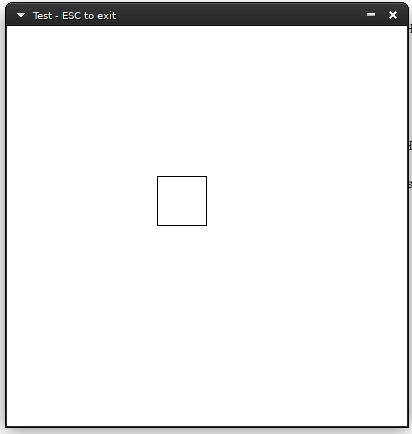
\includegraphics{figures/introduction.png}

\chapter{Bits to byte pixels}
Let's define a way to convert bit information to a byte vector:

\begin{minted}{rust}
pub fn bits_to_bytes(bits: &[u8], width: usize) -> Vec<u32> {
    let mut ret = Vec::with_capacity(bits.len() * 8);
    let mut current_row_count = 0;
    for byte in bits {
        for n in 0..8 {
            if byte.rotate_right(n) & 0x01 > 0 {
                ret.push(BLACK);
            } else {
                ret.push(WHITE);
            }
            current_row_count += 1;
            if current_row_count == width {
                current_row_count = 0;
                break;
            }
        }
    }
    ret
}
\end{minted}

\chapter{Real pixels to byte pixels}
% From graphic gems vol 2 pdf page 109
\skelpars{2}

\chapter{Loading \texttt{xbm} files in \Rust{}}

\texttt{xbm} files are C source code files that contain the pixel information for an image as macro definitions for the dimensions and a static \texttt{char} array for the pixels, with each bit column representing a pixel. If the width dimension doesn't have 8 as a factor, the remaining bit columns are left blank/ignored.

They used to be a popular way to share user avatars in the old internet and are also good material for us to work with, since they are small and numerous. The following is such an image:

\begin{center}

\includegraphics{figures/news.png}
\end{center}
%FIXME
Then, we can convert the \texttt{xbm} file from C to \Rust{} with the following transformations:

\begin{minted}{c}
#define news_width 48
#define news_height 48
static char news_bits[] = {
\end{minted}

to


\begin{minted}{rust}
const NEWS_WIDTH: usize = 48;
const NEWS_HEIGHT: usize = 48;
const NEWS_BITS: &[u8] = &[
\end{minted}

And replace the closing \texttt{\}} with \texttt{]}.

We can then include the new file in our source code:


\begin{minted}{rust}
include!("news.xbm.rs");
\end{minted}

load the image:

\begin{minted}{rust}
let mut image = Image::new(NEWS_WIDTH, NEWS_HEIGHT, 25, 25);
image.bytes = bits_to_bytes(NEWS_BITS, NEWS_WIDTH);
\end{minted}

and finally run it:

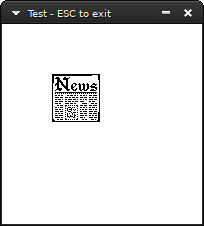
\includegraphics{figures/intro-2.png}

\part{Points and Lines}
\chapter{Distance between two points}

\begin{center}
\input{fig1.pdf_tex}
\end{center}

Given two points, $K$ and $L$, an elementary application of Pythagoras' Theorem gives the distance between them as

\begin{equation}
  r = \sqrt{(x_{L} - x_{K})^{2} +(y_{L} - y_{K})^{2}}
\end{equation}

which is simply coded:

\begin{minted}{rust}
pub fn distance_between_two_points(p_k: Point, p_l: Point) -> f64 {
    let (x_k, y_k) = p_k;
    let (x_l, y_l) = p_l;
    let xlk = x_l - x_k;
    let ylk = y_l - y_k;
    f64::sqrt((xlk*xlk + ylk*ylk) as f64)
}
\end{minted}

\chapter{Distance from a point to a line}
% From graphic gems vol 2 pdf page 40
\skelpars{2}
\chapter{Equations of a line}
\skelpars{2}
\chapter{The parametric form}
\skelpars{2}
\chapter{Angle between two lines}
\skelpars{2}
\chapter{Intersection of two lines}
\skelpars{2}
\chapter{Line through two points}
\skelpars{2}
\chapter{Line equidistant from two points}
\skelpars{2}
\chapter{Normal to a line through a point}
\skelpars{2}
\chapter{Bounding Circle}
% From graphic gems vol 2 pdf page 46
\skelpars{2}
\part{Points, Lines and Circles}
\skelpars{2}
\chapter{Equations of a Circle}
\skelpars{2}
\part{Points, Line Segments and Arcs}
\chapter{Drawing a line segment from its two endpoints}

For any line segment with any slope, pixels must be matched with the infinite
amount of points contained in the segment. As shown in the following figure, a segment \emph{touches} some pixels; we could fill them using an algorithm and get a \bitmap{} of the line segment.

\begin{center}
\input{fig2.pdf_tex}
\end{center}

The algorithm presented here was first derived by Bresenham. In the \emph{Image} implementation, it is used in the \texttt{plot\_line\_width} method.
% From graphic gems vol 1 p 99 (pdf page 124)
%\begin{minted}{rust}
%    pub fn plot_line_width(&mut self,
%                       (mut x0, mut y0): (i64, i64),
%                       (x1, y1): (i64, i64),
%                       wd: f64) {
%        /* Bresenham's line algorithm */
%        let dx = (x1 - x0).abs();
%        let sx = if x0 < x1 { 1 } else { -1 };
%        let dy = (y1 - y0).abs();
%        let sy = if y0 < y1 { 1 } else { -1 };
%        let mut err = dx - dy;
%        /* error value e_xy */
%        let mut e2: i64;
%        let mut x2: i64;
%        let mut y2: i64;
%        let ed: f64 = if (dx + dy) == 0 {
%            1.0
%        } else {
%            f64::sqrt((dx * dx) as f64 + (dy * dy) as f64)
%        };
%        let mut points = vec![];
%        let wd = (wd + 1.0) / 2.0;
%        //eprintln!("wd = {}, ed = {}", wd, ed);
%        loop {
%            points.push((x0, y0));
%            self.plot(x0, y0);
%            e2 = err;
%            x2 = x0;
%            if 2 * e2 >= -dx {
%                /* x step */
%                //eprintln!(" x step ");
%                e2 += dy;
%                y2 = y0;
%                while e2 < ((ed as f64 * wd) as i64)
%                       && (y1 != y2 || dx > dy) {
%                    y2 += sy;
%                    self.plot(x0, y2);
%                    points.push((x0, y2));
%                    e2 += dx;
%                }
%                if x0 == x1 {
%                    break;
%                };
%                e2 = err;
%                err -= dy;
%                x0 += sx;
%            }
%            if 2 * e2 <= dy {
%                /* y step */
%                //eprintln!(" y step ");
%                e2 = dx - e2;
%                while e2 < ((ed as f64 * wd) as i64)
%                       && (x1 != x2 || dx < dy) {
%                    x2 += sx;
%                    self.plot(x2, y0);
%                    points.push((x2, y0));
%                    e2 += dy;
%                }
%                if y0 == y1 {
%                    break;
%                };
%                err += dx;
%                y0 += sy;
%            }
%        }
%    }
%\end{minted}

\section{Faster Drawing a line segment from its two endpoints using Symmetry}
% From graphic gems vol 1 p 103 (pdf page 128)
\skelpars{2}

\chapter{Intersection of two line segments}
\skelpars{2}
% Graphics gems vol 2. pdf page 37
\section{\emph{Fast} intersection of two line segments}
% Graphics gems vol 3. pdf page 231 
\skelpars{2}
\chapter{Printing Line segments With Width}
% Graphics gems vol 1. pdf page 139 "RENDERING FAT LINES ON 2D GRID"
\skelpars{2}
\chapter{Joining the ends of two wide line segments together}
% Graphics gems vol 1. pdf page 132 "AN ALGORITHM FOR FILLING IN 2D WIDE LINE BEVEL JOINTS"
\skelpars{2}
\part{Curves other than circles}
\chapter{Parametric ellipictal arcs}
% Graphics gems vol 3. pdf page 196
\skelpars{2}
\part{Points, Lines and Planes}

\chapter{Union, intersection and difference of polygons}
% Graphics gems vol 2. pdf page 63
\skelpars{2}

\chapter{Centroid of polygon}
% Graphics gems vol 4. pdf page 14
\skelpars{2}

\chapter{Space-Filling Curves}
% Graphics gems vol 2. pdf page 58
\skelpars{2}
\part{Vectors, matrices and transformations}
\chapter{Rotation of a \bitmap{}}

\[
  p' =
  \begin{bmatrix}
    cosθ & -sinθ\\
    sinθ & cosθ
  \end{bmatrix} \]\[ \begin{bmatrix}
    x_{p}\\
    y_{p}
  \end{bmatrix}
\]

\begin{equation*}
  c = cosθ,\\\\
  s = sinθ,\\
  x_{p'} = x_{p}c-y_{p}s,\\
  y_{p'} = x_{p}s+y_{p}c.
\end{equation*}

Let's load an \texttt{xface}. We will use \texttt{bits\_to\_bytes} (See Introduction).

\begin{minted}{rust}
include!("dmr.rs");

const WINDOW_WIDTH: usize = 100;
const WINDOW_HEIGHT: usize = 100;

let mut image = Image::new(DMR_WIDTH, DMR_HEIGHT, 25, 25);
image.bytes = bits_to_bytes(DMR_BITS, DMR_WIDTH);
\end{minted}

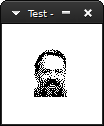
\includegraphics{figures/ch11-1.png}

This is the \texttt{xface} of \texttt{dmr}. Instead of displaying the \bitmap{}, this time we will rotate it $0.5$ radians. Setup our image first:


\begin{minted}{rust}
let mut image = Image::new(DMR_WIDTH, DMR_HEIGHT, 25, 25);
image.draw_outline();
let dmr = bits_to_bytes(DMR_BITS, DMR_WIDTH);
\end{minted}

And then, loop for each byte in \texttt{dmr}'s face and apply the rotation transformation.

\begin{minted}{rust}
let angle = 0.5;

let c = f64::cos(angle);
let s = f64::sin(angle);

for y in 0..DMR_HEIGHT {
    for x in 0..DMR_WIDTH {
        if dmr[y * DMR_WIDTH + x] == BLACK {
            let x = x as f64;
            let y = y as f64;
            let xr = x * c - y * s;
            let yr = x * s + y * c;
            image.plot(xr as i64, yr as i64);
        }
    }
}
\end{minted}

The result:

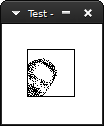
\includegraphics{figures/ch11-2.png}

We didn't mention in the beginning that the rotation has to be relative to a \emph{point} and the given transformation is relative to the \emph{origin}, in this case the upper left corner $(0,0)$. So \texttt{dmr} was rotated relative to the origin\,:
\begin{center}
  \def\svgscale{0.6}
\input{cartesian_grid_dmr_1.pdf_tex}
  \def\svgscale{0.6}
\input{cartesian_grid_dmr_2.pdf_tex}//
(the distance to the origin (actually 0 pixels) has been exaggerated for the sake of the example)
\end{center}

Usually, we want to rotate something relative to itself. The right point to choose is the \emph{centroid} of the object.

If we have a list of $n$ points, the centroid is calculated as:

$$ x_c = \frac{1}{n}\sum_{i=0}^{n} x_i $$
$$ y_c = \frac{1}{n}\sum_{i=0}^{n} y_i $$

Since in this case we have a rectangle, the centroid has coordinates of half the width and half the height.

By subtracting the centroid from each point before we apply the transformation and then adding it back after we get what we want:

Here's it visually: First subtract the center point.

\begin{center}
  \def\svgscale{0.6}
\input{cartesian_grid_dmr_3.pdf_tex}
\end{center}

Then, rotate.

\begin{center}
  \def\svgscale{0.6}
\input{cartesian_grid_dmr_4.pdf_tex}
\end{center}

And subtract back to the original position.

\begin{center}
  \def\svgscale{0.6}
\input{cartesian_grid_dmr_5.pdf_tex}
\end{center}

In code:

\begin{minted}{rust}
let center_point = ((DMR_WIDTH/2) as i64, (DMR_HEIGHT/2) as i64);
for y in 0..DMR_HEIGHT {
    for x in 0..DMR_WIDTH {
        if dmr[y * DMR_WIDTH + x] == BLACK {
            let x = (x as i64 -center_point.0) as f64;
            let y = (y as i64 -center_point.1) as f64;
            let xr = x * c - y * s;
            let yr = x * s + y * c;
            image.plot(xr as i64+center_point.0,
                       yr as i64 + center_point.1);
        }
    }
}
\end{minted}

The result: 
\includegraphics{figures/ch11-3.png}

\section{Fast 2D Rotation}
% Graphics gems vol 1. pdf page 456 
\skelpars{2}
\chapter{90deg Rotation of a \bitmap{} by parallel recursive subdivision}
% Graphics gems vol 2. pdf page 113 
\skelpars{2}
\chapter{Magnification}
\skelpars{2}
\section{Smoothing enlarged \bitmaps{}}
% Graphics gems vol 1. pdf page 189 "SMOOTHING ENLARGED MONOCHROME IMAGES"
\skelpars{2}
\section{Stretching lines of \bitmaps{}}
% Graphics gems vol 3. pdf page 34 "FAST BITMAP STRETCHING"
\skelpars{2}
\part{Flood filling}
\skelpars{2}
% Graphics gems vol 1. pdf page 296 "SEED FILL"
\skelpars{2}
% Graphics gems vol 1. pdf page 299 "FILLING A REGION IN A FRAMEBUFFER"
\skelpars{2}
\part{Areas}
\skelpars{2}
\part{Volumes}
\skelpars{2}
\part{Advanced}
\chapter{Composing monochrome \bitmaps{} with separate alpha channel data}
% Graphics gems vol 3. pdf page 64 "COMPOSING BW BITMAPS
\skelpars{2}
\chapter{Orthogonal connection of two points}
% Graphics gems vol 3. pdf page 205 "SIMPLE CONNECTION ALGORITHM FOR 2D DRAWING"
\skelpars{2}
\chapter{Join segments with round corners}
% Graphics gems vol 3. pdf page 225 "JOINING TWO LINES WITH A CIRCULAR ARC FILLET"
\skelpars{2}
\chapter{Faster line clipping}
% Graphics gems vol 5. pdf page 323 "FASTER PIXEL PERFECT LINE CLIPPING"
\skelpars{2}
\clearpage{}
\bookmarksetup{startatroot}
\colophontitle{About this text}
\pdfbookmark{About this text}{colophon}
\thispagestyle{empty}
\colophontitlesize{25pt}
\begin{colophon}
The text has been typeset in \XeLaTeX{} using the \texttt{book} class and\,:
\begin{itemize}
  \item \textbf{Avara} for the main text.
  \item \emph{\fira{}Fira Sans} for referring to the programming language \Rust{}\,.
  \item \emph{\pixel{}Terminal Grotesque} for referring to the word \bitmap{} as a concept.
\end{itemize}
\end{colophon}
\end{document}
